\documentclass[headings=standardclasses, abstract=true]{scrartcl}

\usepackage{graphicx} % Required for inserting images
\usepackage[sorting=none, style=science]{biblatex} % Required for bibliography
\usepackage{amsmath} % For math equations
\usepackage{minted} % For code blocks
\usepackage[framemethod=TikZ]{mdframed} % For code blocks
\usepackage[svgnames]{xcolor} % For colors
\usepackage{fontspec} % For custom fonts
\usepackage{caption} % For subfigures
\usepackage{subcaption} % For subfigures
\usepackage{float}
\usepackage[
    top=3cm,
    bottom=3cm,
    left=3cm,
    right=3cm
]{geometry} % Required for setting the page size
\usepackage[
    pdfauthor={Sina Atalay},
    pdftitle={RenderCV: A LaTeX CV/Resume App for Academics and Engineers},
    hidelinks=true
]{hyperref} % Required for hyperlinks and metadata

% Path to the bibliography file:
\addbibresource{../docs/assets/bibliography.bib}

% For Python blocks:
\newmdenv[
    outerlinewidth=1,
    outerlinecolor=Gainsboro,
    middlelinewidth=0,
    backgroundcolor=GhostWhite,
    roundcorner=3pt,
    innerbottommargin=12pt,
    innertopmargin=12pt,
    innerleftmargin=12pt,
    innerrightmargin=12pt,
    skipbelow=-0pt
]{pythonbox}
\newfontfamily\vscodefont{Droid Sans Mono}[NFSSFamily=VSCode]
\newcommand{\pythonCodeBlock}[3]{%
    \begin{figure}
        \centering
        \begin{pythonbox}
            \inputminted[fontfamily=VSCode, fontsize=\scriptsize]{python}{#1}
        \end{pythonbox}
        \caption{#2}
        \label{#3}
    \end{figure}
}


\title{\texttt{FastFEM v0.0.1}}
\subtitle{
    A Python package for solving PDEs with the finite element method    \\
    \vspace{0.2cm}
    \href{https://fastfem.com}{fastfem.com}
}
\author{
    Sina Atalay\textsuperscript{1*}, Sacha Escudier\textsuperscript{1*}, Kentaro Hanson\textsuperscript{1*} \\
    {\footnotesize \textsuperscript{1}Princeton University, Princeton, NJ, USA}\\
    {\footnotesize \textsuperscript{*}All authors contributed equally}
}
\date{
    \normalsize December 2024
}


\begin{document}

\maketitle

\begin{abstract}
\noindent Lorem ipsum dolor sit amet, consectetur adipiscing elit. Vestibulum congue gravida sem non dictum. Aenean sit amet mi fermentum ante laoreet dictum sit amet a magna. Praesent sed aliquet dui. Vivamus scelerisque condimentum mauris id euismod. Duis elementum urna eu rutrum mattis. Donec fermentum, risus et viverra aliquet, ante sapien consequat augue, sit amet dictum est nisl id elit. Proin dapibus congue tincidunt. Pellentesque habitant morbi tristique senectus et netus et malesuada fames ac turpis egestas. Fusce felis eros, aliquam sed dui ut, tempor condimentum neque. Donec quis sapien bibendum, faucibus urna sed, gravida felis. Praesent et quam ligula. Aliquam ac est eu odio tincidunt volutpat a in augue. Maecenas fermentum velit felis, vel viverra dui scelerisque pharetra. Nullam eros lorem, finibus pulvinar eleifend eu, pulvinar ac ipsum. Sed velit neque, venenatis sit amet urna vitae, vulputate ullamcorper est.
\end{abstract}

\section{Introduction}

Partial differential equations (PDEs) are the fundamental tools for mathematically modeling natural phenomena. Many fundamental phenomena observed in nature, such as general relativity\supercite{Marolf2001}, quantum mechanics \supercite{Feit1982}, heat diffusion\supercite{Bergman2011}, fluid mechanics\supercite{Lukaszewicz2016}, pricing of financial derivative contracts\supercite{Barles1998}, structural analysis\supercite{Boresi2002}, and electromagnetism\supercite{Griffiths2017}, are described by PDEs. However, most of these PDEs do not have closed-form solutions, especially in complex geometries. Therefore, engineers have developed many numerical methods for solving PDEs. One of the most popular numerical methods among them is the finite-element method (FEM), which originated in the early 1940s\supercite{Liu2022}. FEM is capable of solving non-linear PDEs in highly complex geometries. Since the 1940s, FEM has undergone significant advancements and has revolutionized the way scientific modeling and engineering design. Today, it is widely used in many industrial applications.

Currently, there are many open-source FEM software out there\supercite{fem_getdp, fem_agros, fem_calculix, fem_elmerfem, fem_freefem, fem_goma, fem_fenicsx, fem_dealii}. With \texttt{FastFEM}\supercite{fastfem}, we attempt to develop another open-source FEM software package with the goal of

\begin{itemize}
    \item Creating an easy-to-use and clean Python interface
    \item Using modern tools like JAX\supercite{jax2018github} for advanced array computing with automatic differentiation capabilities
\end{itemize}

One of the motivations for creating a Python interface was the capability of the language to create very intuitive-to-use interfaces. A modern Python interface can offer users a great way of describing FEM problems. The other motivation was leveraging the existing scientific Python environment. Python's popularity in the scientific world is still increasing, and modern libraries with state-of-the-art technologies like JAX, PyVista\supercite{Sullivan2019}, etc., are being developed.


FastFEM is planned to be a big project, but as the goal of \texttt{v0.0.1}, we decided to focus on 2D parabolic PDEs. Parabolic PDEs, such as the heat diffusion equation, Poisson's equation, and the Black-Scholes equation, are very common in various applications. A 2-dimensional parabolic PDE can be expressed as

\begin{equation}
    \frac{\partial^2 f(x,y,t)}{\partial x^2} + \frac{\partial^2 f(x,y,t)}{\partial y^2}
    =
    h(f) \frac{\partial f(x,y,t)}{\partial t} + g(x,y)
    \label{pde}
\end{equation}
where $f(x,y,t)$, $h(f)$, and $g(x,y)$ are scalar functions, $x$ and $y$ are spatial coordinates, and $t$ is time.

Currently, \texttt{FastFEM v0.0.1} can
\begin{enumerate}
    \item create a 2D mesh,
    \item take initial conditions, boundary conditions, h(f), and g(x,y) as inputs,
    \item solve \autoref{pde} with FEM, and
    \item plot the solution.
\end{enumerate}


In this report, the theory behind FEM is summarized. The features and capabilities of \texttt{FastFEM v0.0.1} are presented. Some example results are shown. Finally, the conclusion and outlook are discussed.

\section{Theory}

\section{Features and Capabilities}

This section summarizes \texttt{FastFEM v0.0.1}'s features and capabilities: mesh generation, solving parabolic PDEs with FEM using elements and fields, and plotting.

\subsection{Mesher}

\texttt{FastFEM} uses Gmsh\supercite{Gmsh} for mesh generation. Currently, \texttt{v0.0.1} offers two fundamental 2D mesh generation functions, as shown in \autoref{fig:mesh-example1}.  The results of the functions are shown in \autoref{fig:mesh}. \texttt{FastFEM} is fully statically typed so that users can get autocomplete suggestions when writing the function's arguments and using the mesh object it returns.

\pythonCodeBlock{figures/mesher-example1.py}{Two available functions of \texttt{FastFEM v0.0.1} for generating 2D square and rectangle meshes that are shown in \autoref{fig:mesh}.}{fig:mesh-example1}

\begin{figure}[H]
    \centering
    \hfill
    \begin{subfigure}[c]{0.4\textwidth}
        \centering
        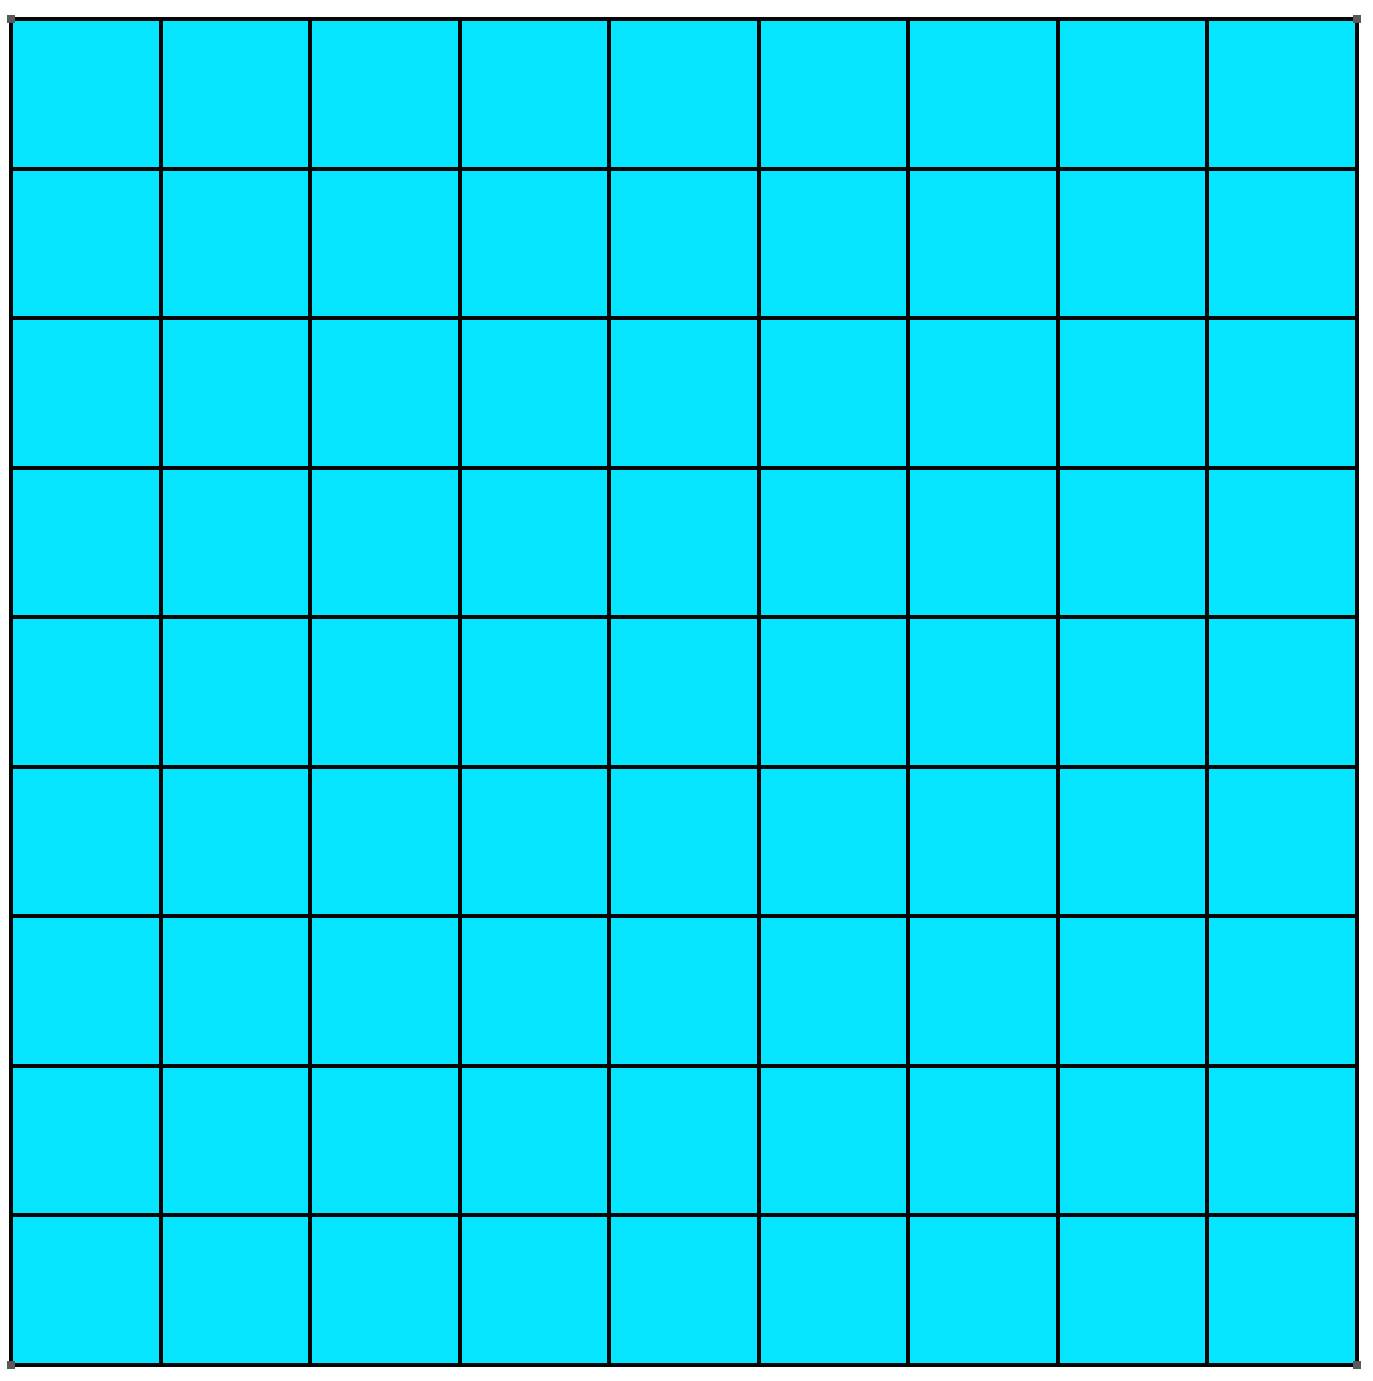
\includegraphics[width=\textwidth]{figures/square_mesh.png}

        \caption{Square mesh.}
        \label{fig:square}
    \end{subfigure}
    \hspace{0.1\textwidth}
    \begin{subfigure}[c]{0.4\textwidth}
        \centering
        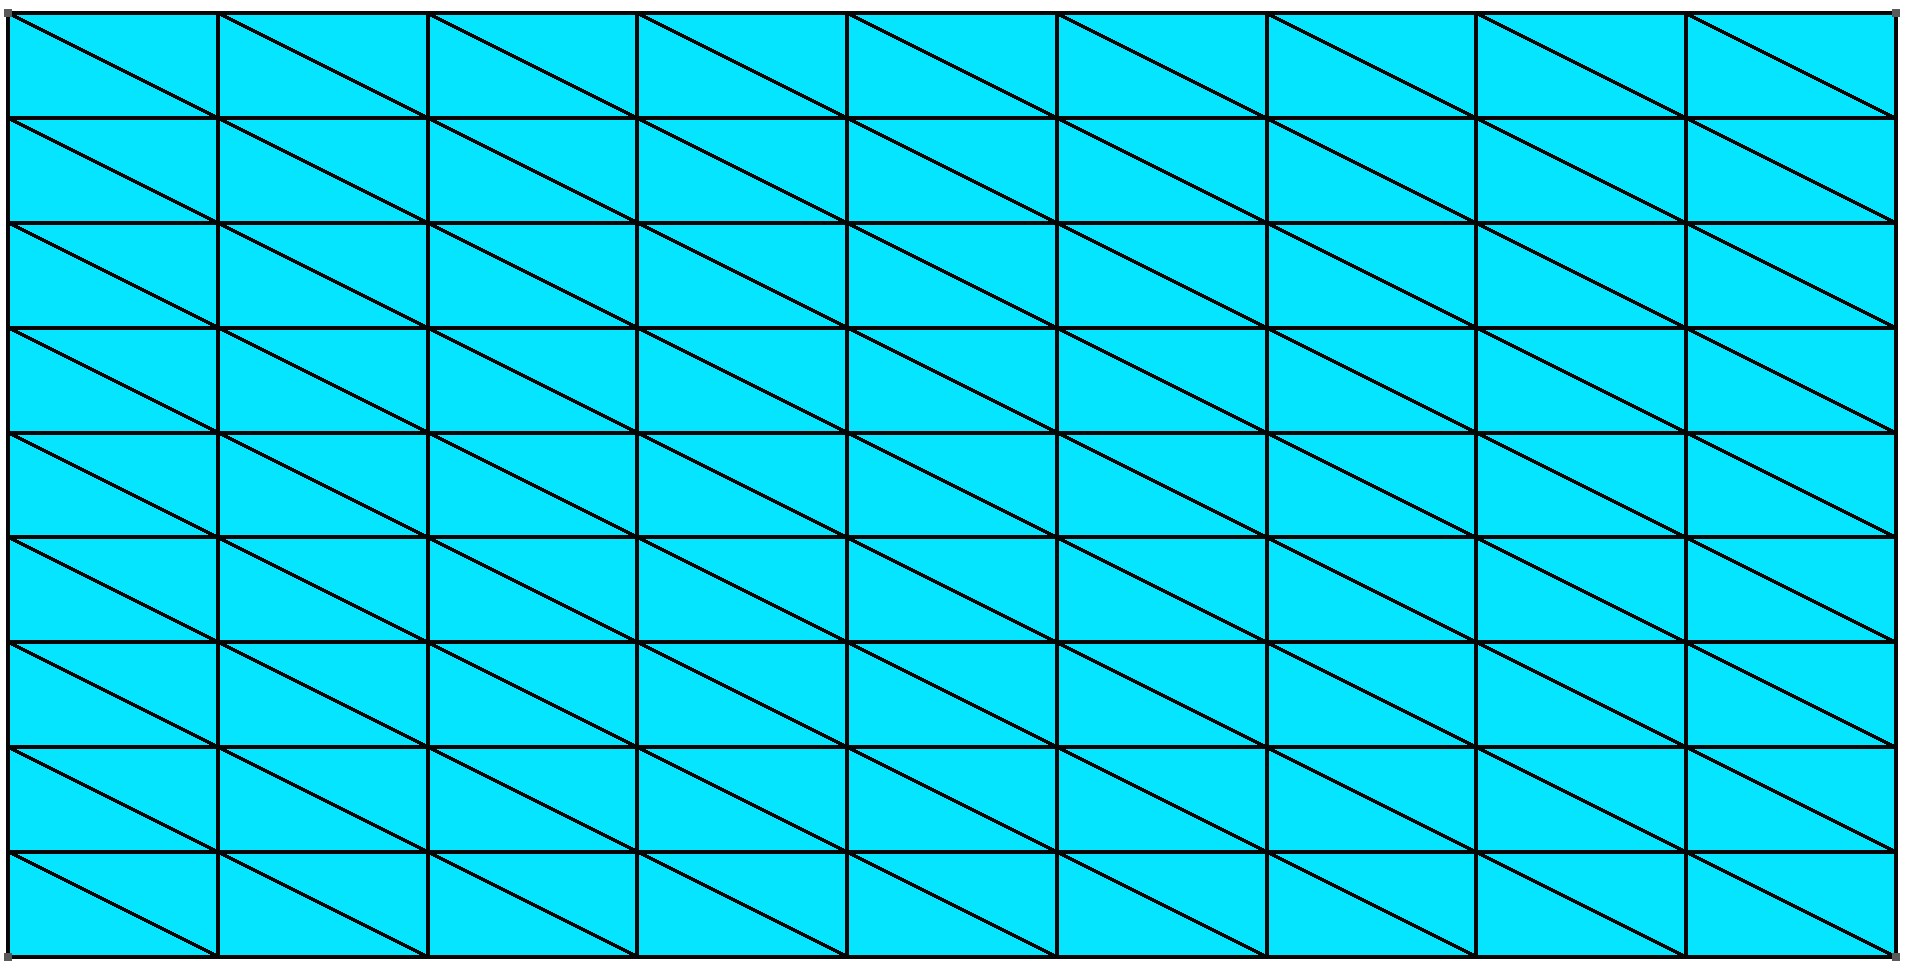
\includegraphics[width=\textwidth]{figures/rectangle_mesh.png}
        \caption{Rectangle mesh.}
        \label{fig:rectangle}
    \end{subfigure}
    \caption{Two examples of mesh generated with the functions in \autoref{fig:mesh-example1}.}
    \label{fig:mesh}
    \hfill
\end{figure}

\texttt{FastFEM v0.0.1} also provides a general-purpose, object-oriented interface for 2D mesh generation by abstracting Gmsh's functional approach. For example, a mesh of an arbitrary 2D geometry, as shown in \autoref{fig:arbitrarymesh}, can be created using the code presented in \autoref{fig:mesh-example2}.

\pythonCodeBlock{figures/mesher-example2.py}{The code that generates the mesh of an arbitrary geometry shown in \autoref{fig:arbitrarymesh}.}{fig:mesh-example2}

\begin{figure}[H]
    \centering
    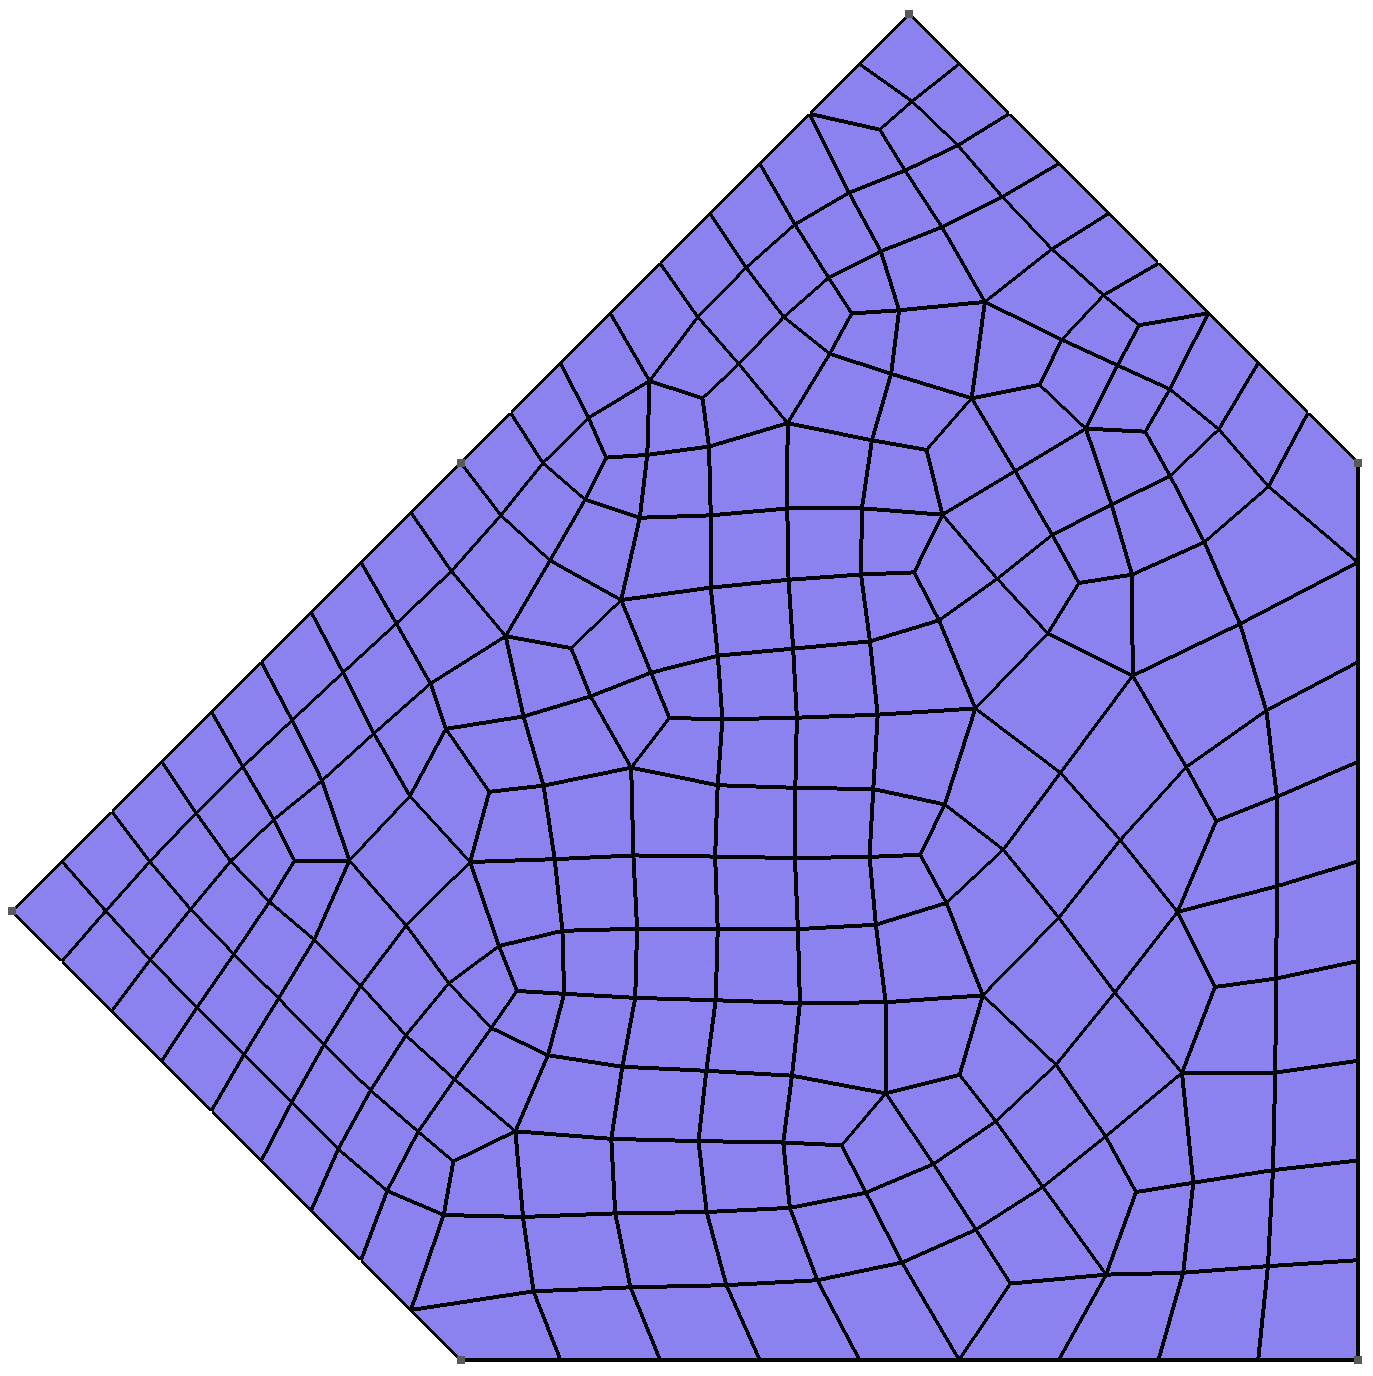
\includegraphics[width=0.5\textwidth]{figures/arbitrary_mesh.png}
    \caption{An arbitrary 2D mesh generated using the code in \autoref{fig:mesh-example2}.}
    \label{fig:arbitrarymesh}
\end{figure}

\subsection{Elements and Fields}

\subsection{Plotter}

\texttt{FastFEM} uses \texttt{PyVista}'s (insert source here) plotting capabilities for visual representation. There are currently six methods available to the user:

\begin{itemize}
    \item \texttt{define\_plotter()}: This is a helper method, responsible for interfacing the mesh object as produced by the mesher to \texttt{PyVista}'s own requirements. Notably, it returns a PyVista grid object containing all relevant information on the nodes and connectivity of the mesh, and is subsequently used for plotter generation.
    \item \texttt{plot\_mesh()}: This method is responsible for plotting the mesh object, and confirming \texttt{PyVista}'s redering is correct. In addition, it has aethetics related parameters that can be switched to the user's liking.
    \item \texttt{plot\_data()}: This method will plot the data on a mesh, without any time dependency. It is intended to either plot a single frame of the equation \ref{pde}, of its steady-state solution.
    \item \texttt{animate\_data()}: This method will plot the time-dependent data in an interactive window, such that the user can directly test the quality of their mesh/validity of their data.
    \item \texttt{make\_movie()}: This method will output a .mp4 file of the time-dependent data.
    \item \texttt{make\_gif()}: This method will output a .gif file of the time-dependent data.
\end{itemize}

Of most notable note, the interactive widnow generated by \texttt{plot\_mesh()} will strongly resemble the output as shown in figure \ref{fig:mesh}, but with higher customizability. A sample output is given in figure \ref{fig:PyVistaMesh}.

\begin{figure}[H]
    \centering
    \hfill
    \begin{subfigure}[c]{0.3\textwidth}
        \centering
        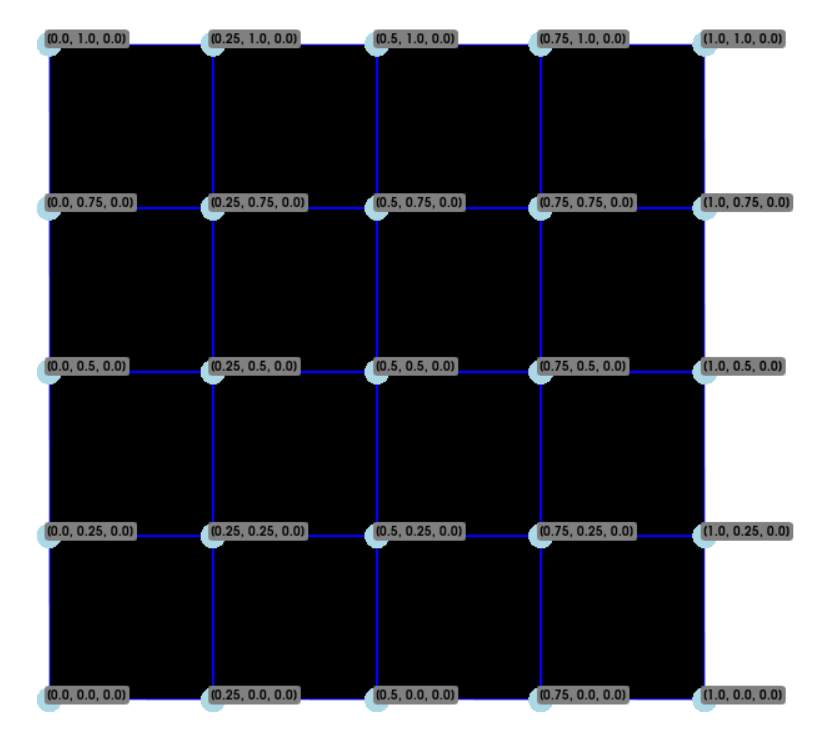
\includegraphics[width=\textwidth]{figures/PyVistaMesh_Customized.png}
        \caption{Ordered mesh, with quadrangles.}
        \label{fig:PyVistaMesh1}
    \end{subfigure}
    \hspace{0.1\textwidth}
    \begin{subfigure}[c]{0.4\textwidth}
        \centering
        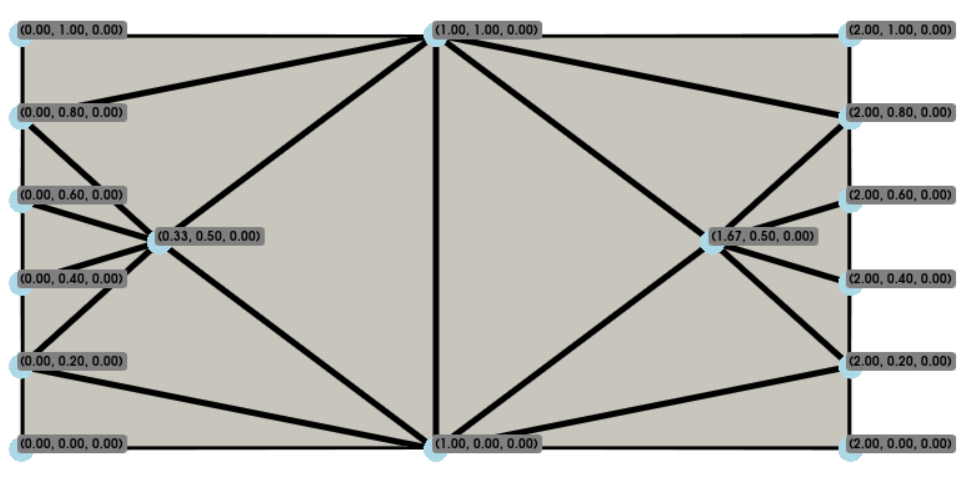
\includegraphics[width=\textwidth]{figures/PyVistaMesh_Customized2.png}
        \caption{Disordered mesh, with triangles.}
        \label{fig:PyVistaMesh2}
    \end{subfigure}
    \caption{Mesh outputs of \texttt{plot\_mesh()}, using \texttt{PyVista}'s rendering capabilities.}
    \label{fig:PyVistaMesh}
    \hfill
\end{figure}

Where the user may also interact with the mesh, and rotate it to any angle. 

In addition, a single frame may also be plotted using the \texttt{plot\_data()} method, given the PDE has already been solved separately, and the content of each node in stored in a 3-dimensional array, for each time-step of the simulation. A sample output is given in figure \ref{fig:PyVistaPlotFrame}.

\begin{figure}[H]
    \centering
    \hfill
    \begin{subfigure}[c]{0.4\textwidth}
        \centering
        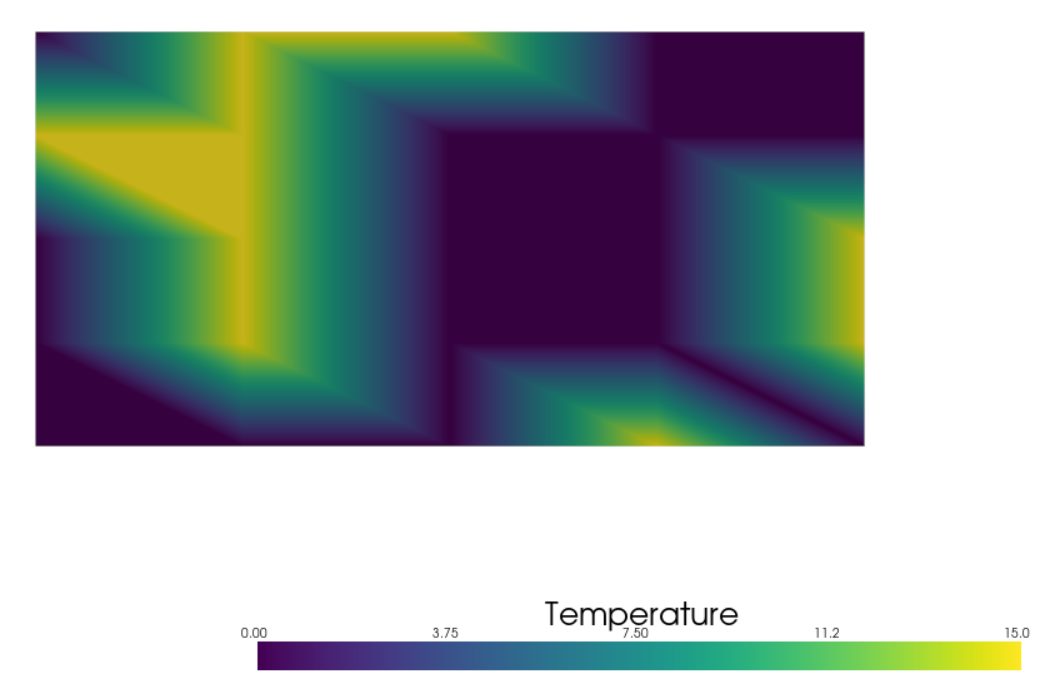
\includegraphics[width=\textwidth]{figures/PyVistaMesh_32.png}
        \caption{Plotted sample data, with 32 elements.}
        \label{fig:PyVistaMesh1}
    \end{subfigure}
    \hspace{0.1\textwidth}
    \begin{subfigure}[c]{0.4\textwidth}
        \centering
        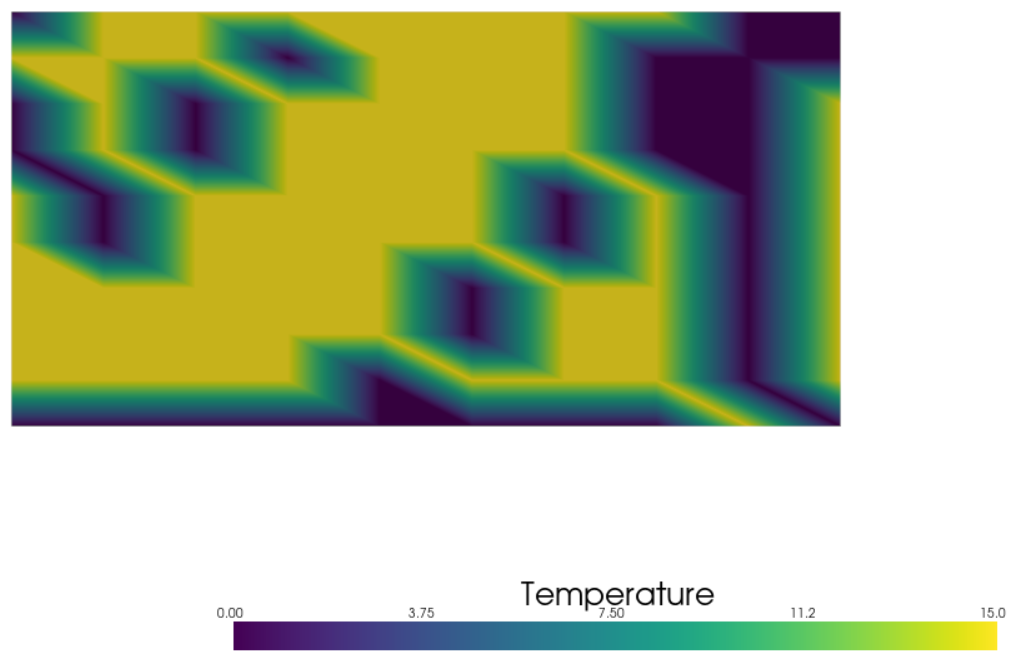
\includegraphics[width=\textwidth]{figures/PyVistaMesh_162.png}
        \caption{Plotted sample data, with 162 elements.}
        \label{fig:PyVistaMesh2}
    \end{subfigure}
    \caption{Outputs of \texttt{plot\_data()}.}
    \label{fig:PyVistaPlotFrame}
    \hfill
\end{figure}

Where the change in the number of elements accurately represents an increase in the resolution and quality of the solution.

In addition, another capability added by the \texttt{plotter} branch is the ability to animate the data interactively, and subsequently save a movie or gif of such data. A sample output is given in figure \ref{fig:PyVistaAnimated}.

\begin{figure}[H]
    \centering
    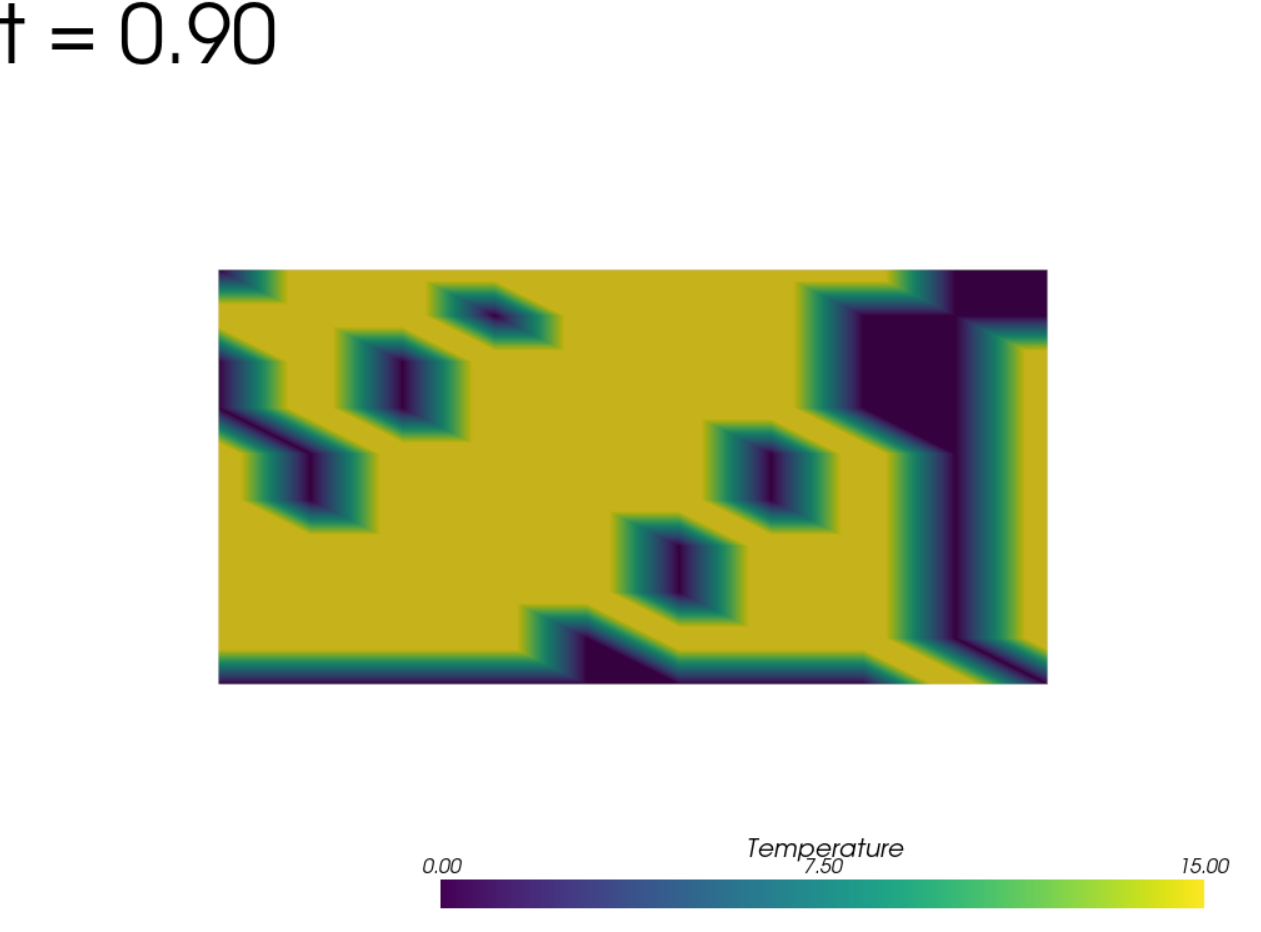
\includegraphics[width=0.5\textwidth]{figures/PyVista_Animated.png}
    \caption{A single frame of the animated data.}
    \label{fig:PyVistaAnimated}
\end{figure}

Where the most notable difference with the \texttt{plot\_data()} method is the plotted time at the top-left corner of the figure. In addition, using the \texttt{animate\_data()} method, the user has control over the number of frames per second of the animation, and enhance readability of the solution.

\textbf{Note}: Throughout the development of the \texttt{plotter} branch, testing remained a difficult aspect of the project. Many of the methods use rely on visual cues and generated plots to understand their validity. As such, the evaluation of the methods relied primarily in the assertion of the \textit{creation} of the method, rather than its actual content. To achieve this, \texttt{PyVista}'s show method (responsible for actually outputting the plot) was mocked using \texttt{unittest} and the \texttt{MonkeyPatch} testing fixture, such that no plot was actually generated thorugh the tests.

Another particular difficulty lied in the testing of the \texttt{make\_movie()} and \texttt{make\_gif()} methods, due to incompabilities of file writing across different operating systems and their reliance on external libraries, which resulted in tests passing locally but not through GitHub's CI pipeline. As such, these tests are currently skipped, while the issue is being actively debugged.




\section{Results}

\section{Software Quality and Maintenance}

\texttt{FastFEM} is open-source and version-controlled on GitHub\supercite{fastfem}. We are following some rules to ensure high software quality for better maintainability:

\begin{itemize}
    \item Direct pushes to the "main" branch are not allowed. All the contributions should be made as a pull request.
    \item Each pull request should be reviewed by two developers, and all the automated tests should be passed before it is merged.
    \item All the documentation and reports related to the software are maintained in the same repository.
    \item All the important discussions are conducted on the issues page.
    \item The changelog is kept.
    \item Semantic Versioning 2.0.0\supercite{semanticVersioning} convention is followed for versioning.
\end{itemize}

\texttt{FastFEM} also uses many other open-source tools for various reasons:
\begin{itemize}
    \item Hatch\supercite{hatch} is used as a project manager.
    \item MkDocs\supercite{mkdocs} with Material theme\supercite{mkdocsmaterial} is used for the documentation.
    \item MkDocstrings\supercite{mkdocstrings} is used to generate API references.
    \item pytest\supercite{pytest} is used to write automated tests.
    \item GitHub Actions\supercite{githubactions} is used to run the automated tests after each update.
    \item pre-commit\supercite{precommit}, Ruff\supercite{ruff}, and Black\supercite{black} are used for linting and formatting.
    \item pre-commit.ci is used to run the linters and formatters after each update.
\end{itemize}


\section{Conclusion and Outlook}

\clearpage
\printbibliography

\end{document}